\documentclass[11pt]{article}

\usepackage{graphicx}
\usepackage{amsfonts}
\usepackage{amsmath}
\usepackage{amsthm}
\usepackage{latexsym}
\usepackage{amssymb}
\usepackage{hyperref}

\pagestyle{plain}
\bibliographystyle{plain}

\title{DATA ENCRPTION STANDARD}
\author{}

\begin{document}

\maketitle

\section{Introduction}

\subsection{Cryptography}
\quad\quad Cryptography is practice and study of techniques for secure communication in insecure  networks.
The Word “cryptography” is derived form Greek words ‘kryptos’ (hidden) and ‘graphein’ (write).
\cite{Intro}
It uses mathematical techniques to encrpt and decrypt data.
In recent times,Cryptography is every where 
In Secure Communications  i.e,  in web traffic (HTTPS) and  wireless (GSM,Bluetooth).
 It is used for files on disk (EFS,TrueCrypt) and for Content protection like DVD, Blueray (CSS,AACS) and more.
 \subsubsection{History}
\quad\quad The first known use of cryptography is found in non-standard hieroglyphs which is an inscription carved into the wall of a tomb around 1900 B.C in Egypt.\\
 There are three era's in cryptography:\\
 1.Manual Era\\
 2.Mechanical Era\\
 3.Modern Era\\
 
 
 $\blacktriangleright${Manual Era}\\
 
    \quad In this era,there was only usage of pen and paper i.e,everything was done manually. The first inscription also comes under this. 
    Later, there were many forms that came into existence like Scytale, Atbash, Caesar.\\
         
         \quad SCYTALE is a tool used to perform a transposition cipher.It consists of a cylinder with a strip of parchment wound around it on which a message is written.The ancient Greeks and the Spartans in particular used this cipher to communicate during military campaigns.The recipient uses a rod of the same diameter on which the parchment is wrapped to read the message. It has the advantage of being fast and not prone to mistakes—a necessary property when on the battlefield. 
However,It can be easily broken.Since the strip of parchment hints strongly at the method,the ciphertext would have to be transferred to something less suggestive,somewhat reducing the advantage noted.\\
     
     
        ATBASH cipher is a very specific case of a substitution cipher where the letters of the alphabet are reversed. 
In otherwords, all As are replaced with Zs, all Bs are replaced with Ys, and so on.
Because reversing the alphabet twice will get you actual alphabet, you can encipher and decipher a message using the exact same algorithm.\\
{\bf Example:}\\
Plaintext: This is a secret message\\
Ciphertext: Gsrh rh z hvxivg nvhhztv\\
        
        CAESAR cipher is a substitution cipher where each letter in the original message is replaced with a letter corresponding to a certain number of letters up or down in the alphabet.
 The most used number was 3.The caesar cipher is also called as shift cipher.This is the most simplest forms of encryption.\\
 {\bf Example:}\\
 Plaintext: Attack\\
 Ciphertext: dwwdfn\\
 
$\blacktriangleright${Mechanical Era}\\
 
        \quad Use of machines for encryption started in 18th century during this era. 
Many machines were made at that time.some of them are Deisus Wadsworth(1817), Jefferson’s encryptor and many more.In those the most used and Well reputed machine was Enigma(1920).\\

$\blacktriangleright${Modern Era}\\
         
        \quad This era of cryptography refers to computers. There are many number of cryptosystems that came into existence like RSA, DES, AES and more.\\

\cite{Intro}



\subsubsection{Types of Cryptography}

 SYMMETRIC CRYPTOGRAPHY:\\
 
 In symmetric cryptography,we use the same key for encryption and decryption.It can be divided into two categories,\\
$\blacktriangleright$Stream Ciphers\\
       These can encrypt a single bit or byte of plaintext at a time.\\
$\blacktriangleright$Block Ciphers\\
       These take a number of bits and encrypt them as a single unit which is called as a block.Usually,the block size can be 64,128 or 256 bits.\newline
\newline
ASYMMETRIC CRYPTOGRAPHY:\\

In Asymmetric cryptography,we use a public key for encryption and a private key for decryption.Asymmetric cryptography is also called as Public key cryptography.\\


\subsection{DES}

\quad\quad The Data Encryption Standard (DES) is a symmetric-key algorithm for the encryption of electronic data. Although now considered insecure, It was highly influential in the advancement of modern cryptography.It is a block cipher.

\subsubsection{History of DES}

\quad\quad The origins of DES go back to the early 1970s. In 1972, after concluding a study on the US government's computer security needs, the US standards body NBS(National Bureau of Standards) now named NIST(National Institute of Standards and Technology) identified a need for a government-wide standard for encrypting unclassified,sensitive information.
Accordingly, on 15 May 1973, after consulting with the NSA,NBS solicited proposals for a cipher that would meet rigorous design criteria. None of the submissions,however,turned out to be suitable.A second request was issued on 27 August 1974. 
This time, IBM submitted a candidate which was deemed acceptable,a cipher developed during the period 1973–1974 based on an earlier algorithm, Horst Feistel's Lucifer cipher.\\
$\rightarrow${In 1970’s,IBM created a crypto system called “Lucifer” for encryption of customers data.}\\
$\rightarrow${In 1973, NIST made a proposal for national symmetric key cryptosystem.}\\
$\rightarrow${IBM submitted Lucifer for validation.}\\
$\rightarrow${Later on, changes were made by Walter Tuchman and that was accepted and called as DES.}\\
$\rightarrow${DES is a symmetric block cipher, it encrypts 64 bits plain text with 64 bit key at a time.}\\\cite{His}



\section{Background}
Note:Please refer \cite{back} and \cite{back2} for more information on permutations and XOR.
\subsection{Notation}

\quad\quad XOR is a connective in logic which is known as "exclusive disjunction" or "exclusive or".It is true only when one of the two conditions is true.It is used for bitwise operations.\\
  It works on these rules,\\
  1$\oplus$1 = 0\\
  1$\oplus$0 = 1\\
  0$\oplus$1 = 1\\
  0$\oplus$0 = 0\\
 Here 0 means false,1 means true.\\
{\bf Example:}\\
    0101\\
    0110\\
XOR-0011\\
The result is 0011.

\subsection{Permutation}

\quad\quad Permutation is the process of rearranging the bits in specified order.
The number of permutations on a set of n elements can be given by n!.\\
{\bf Example:}\\
2!=2.1=2 permutations of {1,2} i.e, {1,2} and {2,1}.

\section{The DES Cryptosystem}
\subsection{Description}
\qquad\quad The DES is a block cipher.It encrypts data in 64-bit blocks.this is a symmetric algorithm.
A 64-bit block of plaintext goes in one end and a 64-bit block of ciphertext comes out the other end.Here,same algorithm and key are used for encryption and decryption.

\quad\quad The key length is 56-bits.The key is usually expressed as a 64-bits,but every eighth bit is used for parity checking and is ignored.These parity bits are the least significant bits 
of the key bytes.The key can be any 56-bit number and can be changed at anytime.

\quad\quad The DES is a combination of a substitution followed by a permutation on the text,based on the key.This is known as a round.DES has 16 fiestel rounds,It applies the same combination
of techniques on the plaintext 16 times.

\subsection{Working of DES}
\qquad\quad DES operates on a 64-bit block of plaintext.After an initial permutation,the block is made into right half and left half each 32bits long.
In each round, the key bits are shifted,and then 48 bits are selected from 56 bits of the key.The right half of the data is expanded to 48 bits through an expansion permutation,
combined with 48 bits of a shifted and permuted key through an XOR,sent through 8 S-boxes producing 32 new bits,and permuted again.These four functions make Function f.

\quad\quad The output of function f is then combined with the left half via another XOR.The result of these operations becomes the new right half and the old right half becomes the new left half.
These operations are repeated for 16 times.

\begin{figure}
\begin{center}
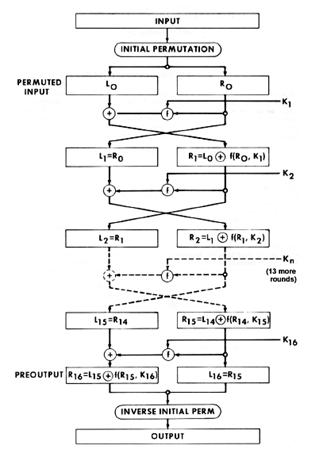
\includegraphics[scale=0.9]{des.jpg}
\end{center}
\caption{DES}\label{Working of DES}
\end{figure}
This is areference to Figure~\ref{Working of DES} \cite{source2}
\\The DES encryption process consists of three main steps:\\
$\blacktriangleright${Initial Permutation}\\
$\blacktriangleright${16 Fiestal Rounds}\\
$\blacktriangleright${Final Permutation}\\
\\INITIAL PERMUTATION:

Initial Permutation occurs before round 1,it transposes the input block.For example,the initial permutation moves bit 58 of the plaintext to bit position 1,
bit 50 to bit position 2 and so on.

     In the fiestel round,the input is expanded and XORed with key and again compressed to its original size.
     Here the 32-bit input is expanded to 48-bit using expansion permutation by duplicating half of the bits.
     For each 4-bit input block,the first and fourth bits each represent two bits of the output block,while the second and third bits each represent one bit of the output block.
     For example,the bit in position 3 of the input block moves to position 4 of the output block and the bit in position 21 of the input block moves to positions 30 and 32 of the 
     output block.

\begin{figure}     
\begin{center}
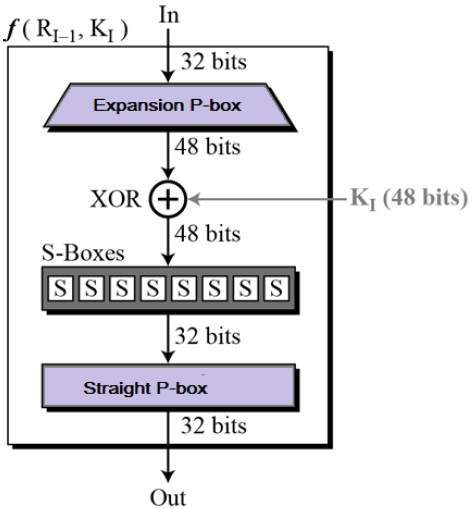
\includegraphics[scale=0.3]{round_function.jpg}
\end{center}
\caption{Expansion Box.}\label{Fiestal Round}
\end{figure}
This is a reference to Figure~\ref{Fiestal Round} \cite{source1}

\subsubsection{The Key Generation}
  
\qquad\quad Initially,the 64-bit DES key is reduced to a 56-bit key by ignoring every eighth bit.These bits can be used as parity check to ensure the key is error-free.
  After the 56-bit key is extracted,a different 48-bit subkey is generated for each of the 16 rounds of DES.
  
\quad\quad Firstly,the 56-bit key is divided into 28-bit halves.Then,the halves are circularly shifted by either one or two bits,depending on the round.
  After being shifted,48 out of the 56 bits are selected.Because this operation permutes the order of the bits as well as selects a subset of bits,
  It is called as compression permutation.\\
  Eventually,16 keys are generated and are saved for each fiestel round.

 
\subsubsection{The S-box Substitution}
This is a reference to Figure~\ref{S-boxes} \cite{source4}

\quad\quad After the compressed key is XORed,the 48-bit result moves to a substitution operation.The substitutions are performed by eight substitution boxes.Each S-box has a 6-bit input and a 4-bit 
output.There are 8 different S-boxes.The 48-bits are divided into eight 6-bit sub-blocks.The first block is operated by S-box 1,the second by S-box 2 and so on.Each S-box is a table of 4 rows 
16 columns.each entry in the box is a 4-bit number.The output can be known by looking the row and column number specified by 6 input bits of the S-box.\\
  \begin{figure}   
 \begin{center}
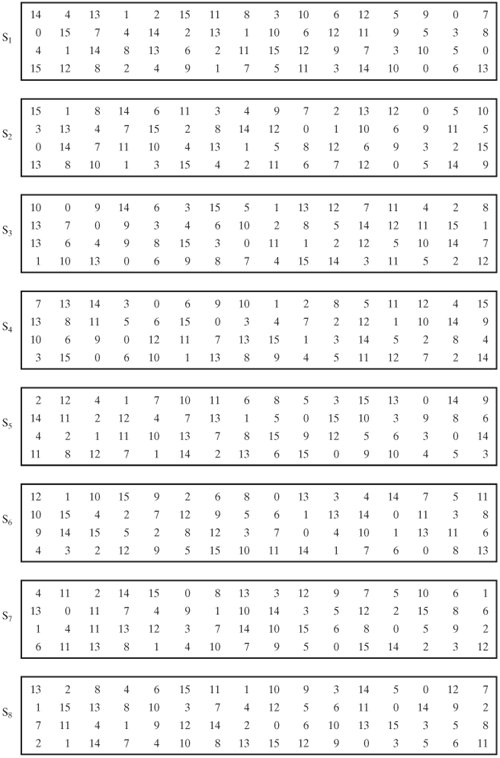
\includegraphics[scale=0.5]{s_boxes.jpg}
\end{center}
\caption{S-boxes.}\label{S-boxes}
  \end{figure}
\quad\quad An entry in the S-box is specified by input bits in a particular manner.Consider an S-box which has input of 6 bits labelled as m1,m2,m3,m4,m5 and m6.Now,m1 and m6 are combined to 
form 2-bit number which corresponds to a row in the table. and the middle bits m2 to m5 are combined to form a 4-bit number which corresponds to column in the table.
  For example,Consider 6 bits 111000.
 

\quad\quad Here the first and last bit are combined and the row value is "10" which is 3 and the middle 4 bits are combined,the column value is "1100" which is 10.
Now,we check the value in third row and tenth column in the table which is 9(1001).

\quad\quad The result of this S-boxes will be eight 4-bit blocks which are recombined into a single 32-bit block.
    The 32-bit output of the S-box substitution is permuted according to a P-box.This permutation maps each input bit to an output position.This is called as straight permutation 
 or a permutation.Here no bits are used twice and no bits are ignored.For example,bit 4 moves to 31 and bit 2 moves to 28 and so on.\\
\\FINAL PERMUTATION:

\quad\quad The final permutation is the inverse of the initial permutation.After the last round of DES,the left and right halves are not exchanged.
The last output is used as the input for final permutation.
Then we exchange the halves and shift around the permutation and exactly the same result is obtained.

 
\subsubsection{DECRYPTION}
  \qquad\quad This is exactly the reverse functioning of encryption.The keys we use for encryption are stored and are used in the reverse order.
  Final permutation will be the initial permutation and Initial permutation will be the final permutation.For suppose,the encrytion keys for each round are k1,k2,...,k16 then
the decryption keys for each round are k16,k17,....k1.the algorithm that generates the key used for each round is circular as well.

\section{Implementation}

\quad\quad Converting Binary to Hexadecimal- method used is inptobin().
After taking 16 bit hexa decimal input message or key it would be converted to binary.

Encryption starts with  method expand().
Here,initial permutation is done using the array initialper[].
Binary Message is devided into two equal halfs 32 bit each right and left,
64 bit key is converted to 56bit by using array PC1[] and divided into two halfs.

Later,the key is generated using key() method .
Here,the two halfs undergoes shifting operation based on array rotations[].
Then,the key is compresed to 48bit using PC2[] array.
And the generated key is stored in every round.

Now the right half of input and key XOR operation done using xor() method.
Here the 32 bit input is expanded to 48 bit using aray EBIT[].
Then,it is XORed with key single bit at a time.

S-Box operation is doen using sblock() method.
Here,the 48 bit input from XOR is to be compressed to 32 bit.
Here,there are 8 S-Boxes are used to achieve the required operation, using 6 bits for each 8bit.
S-boxes are stored in 2dimensional array S[][].
The values in s-box across the row and column of the 6bit used are converted to 4bit binary.
Total 8 4bit blocks make 32 bit.

Next the output from s-boxes is XORed with Left input, and switching left and right achieved using newLRbits() method.
Here,the binary is coverted to HexaDecimal.

Decryption is done using decrypt() method.
This is exactly the reverse of Encryption.Firstly,we collect the stored key from last position by using array Key[].
Then,we reverse the process through S-box and the binary bits are appended to the output.Now,the P table is applied to
the output and this is the final output of one S-box round.Later on,we swap the right and left bits then 
convert the input to binary and then finally,initial permutation is performed and we get the desired output.




   

\section{Conclusion}
 \quad\quad After many years,DES was breaked by many attacks such as brute force,differential cryptanalysis and linear cryptanalysis.Then,Triple DES came into existence which 
is nothing but applying DES 3 times which was considered slow.
Later On,AES which is called as Advanced Encryption Standard was invented.It is also a block cipher but uses 128-bit blocks and is more effective than DES.
  
\bibliography{desprjct}
\end{document}
      
      
